\begin{figure}[t!]
\centering
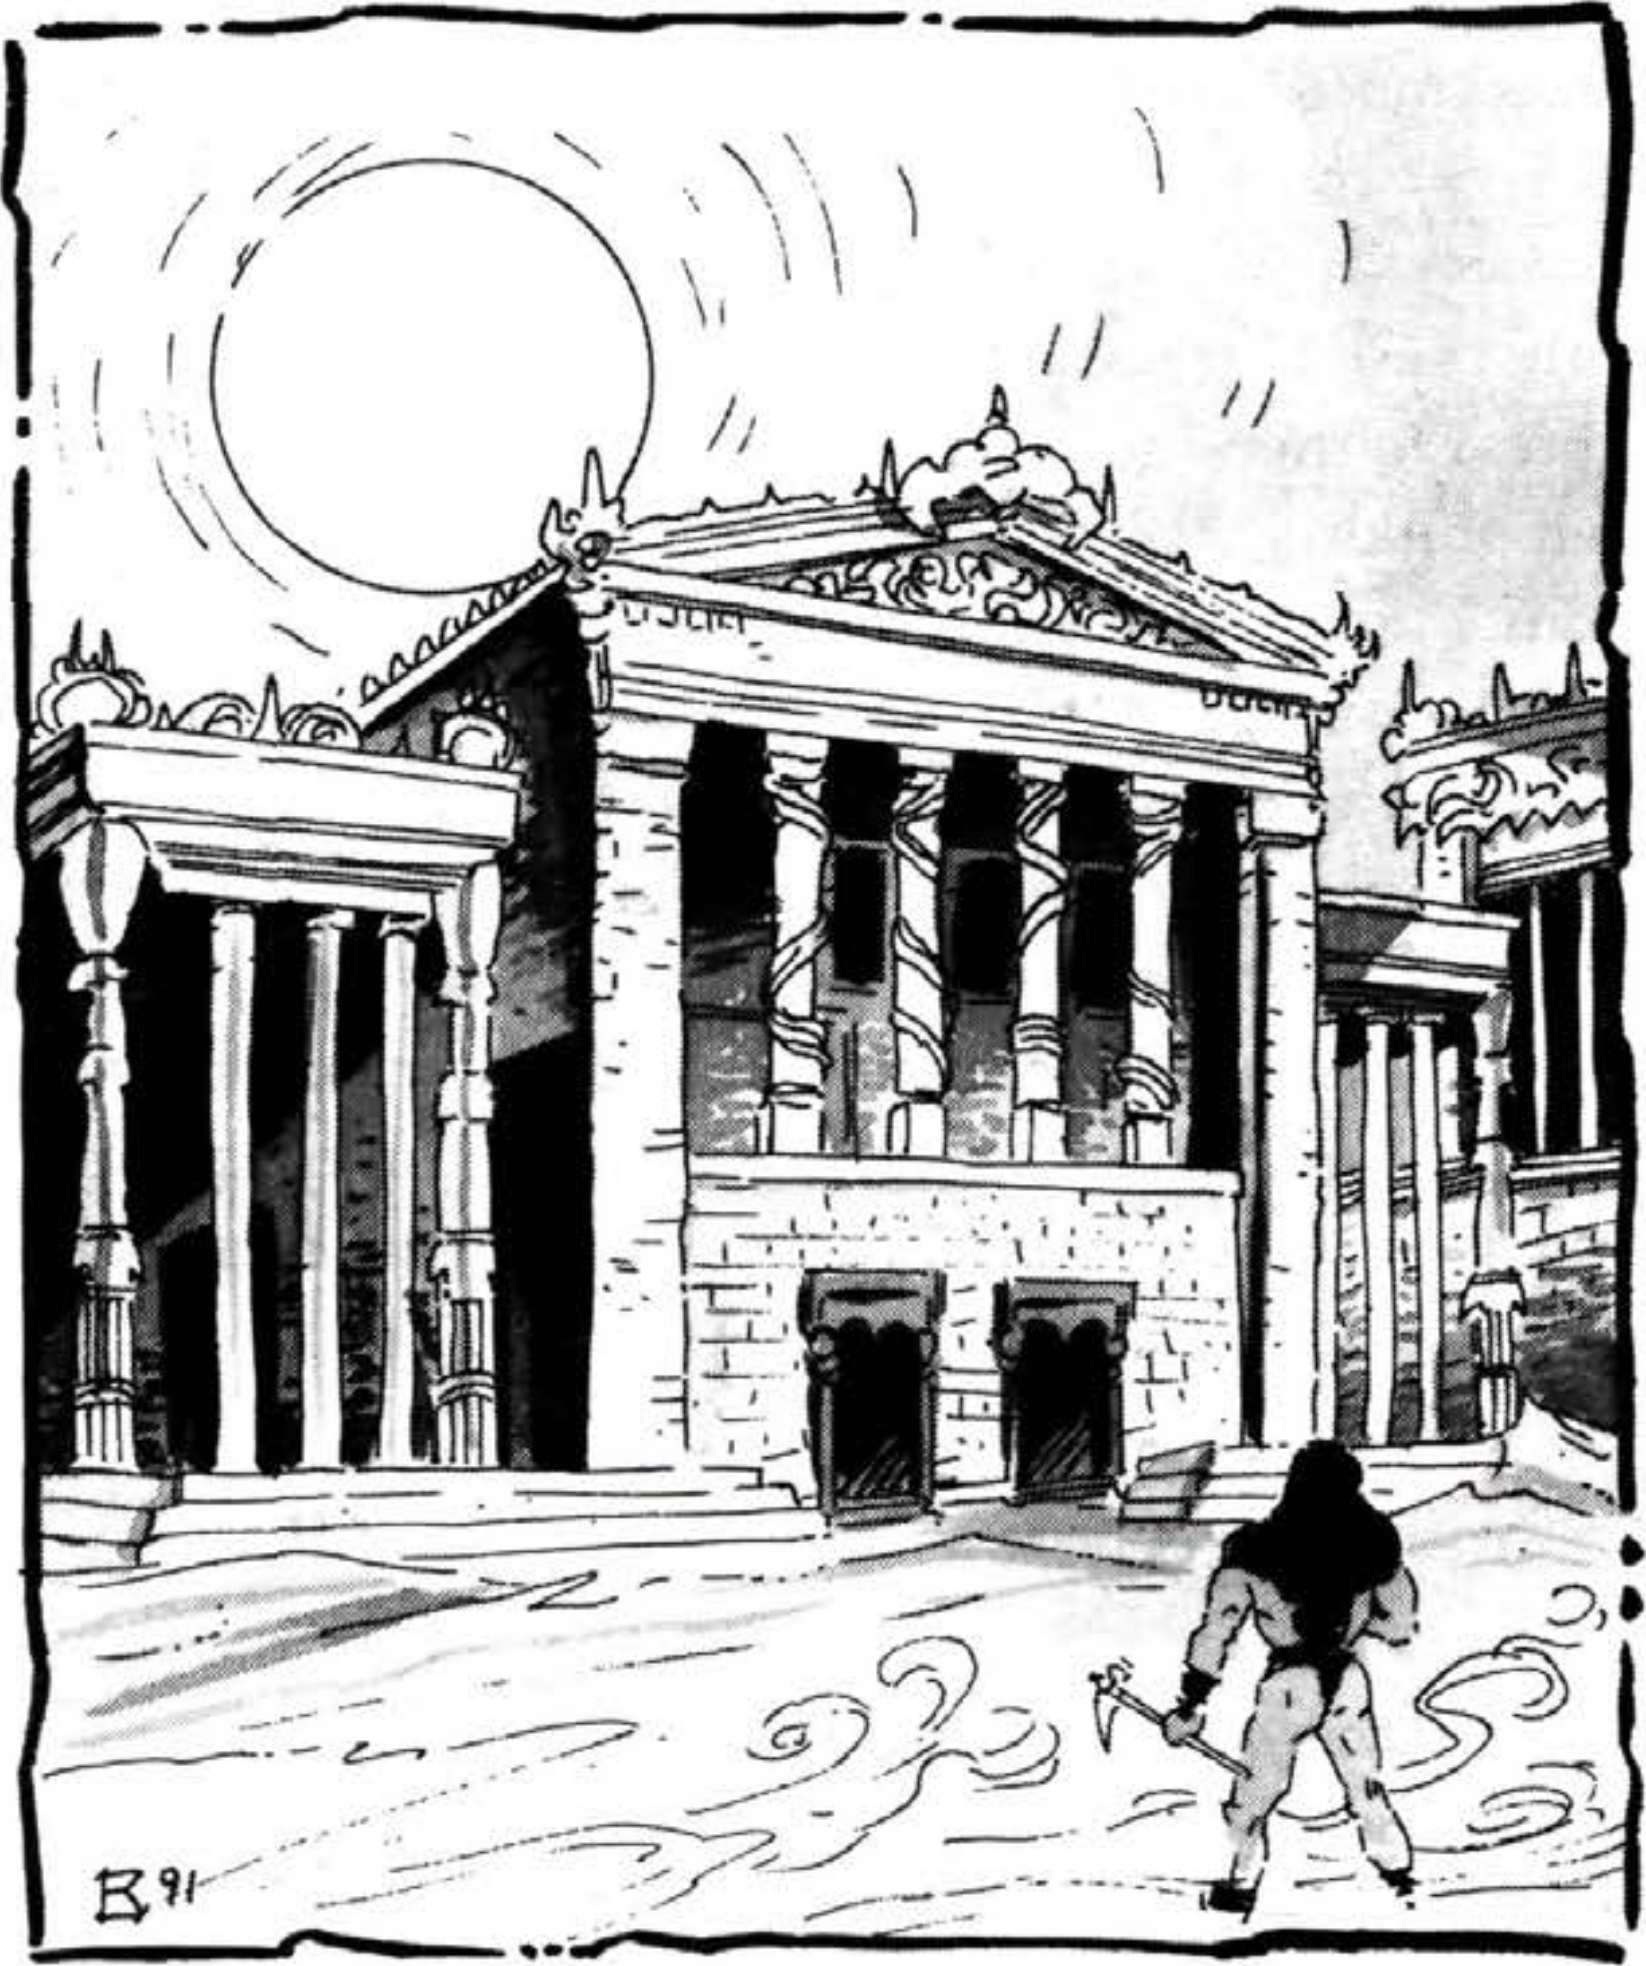
\includegraphics[width=\columnwidth]{images/balic-1.png}
\end{figure}

\City{Balic}
{28,000 (78\% humans, 8\% dwarves, 4\% elves, 4\% half-giants, 3\% muls, 2\% thri-kreen, 1\% other).}
{Grain, salt, olives, kank nectar, leather, livestock, silver.}
{Common, Dwarven, Elven, Balikite.}
{
	The sorcerer-king Andropinis once ruled Balic from the airy confines of the White Palace, not far from the dusty shores of the city's silt harbor. One day in the Year of Friend's Agitation (FY 10), he boarded his silt armada and struck out for the far side of the Sea of Silt. It was a trip from which he never returned.

	Balic has suffered on a number of fronts in recent years. In the Year of Dragon's Agitation (FY 3), when Tyr had refused to pay the Dragon's Levy, it fell to Balic to make up the loss by adding an extra thousand slaves to its contribution. The following year, Mountain's Fury, saw the Peninsula Rampage, a short-lived war in which a small army of giants overran most of the Balican Peninsula. Half of Balic's army and a quarter of its fields were destroyed in the battle. The city-state was still recovering when Andropinis fell to Rajaat's revenge a few years later.
}
{
	Balic is a clean, comfortable metropolis on the shores of a silt bay. Since Andropinis' disappearance, the city has been divided into three parts, each ruled over by a different trade lord. Balic was untouched by the Great Earthquake, but other disasters have left their marks on the place in recent years. For the most part, however, life under the trade lords is considerably better than it was under the cruel and oppressive Andropinis.

	Even the territory controlled by House Tomblador, whose lord attempts to pattern himself as Balic's new dictator, is pleasant compared to the atrocities of the previous ruler.

	On the surface, the city appears to be one sprawling metropolis, not a divided city. No walls separate one territory from another, no guards wait to collect tolls as citizens move from block to block. To the locals, however, there is a clear delineation between one lord's domain and the next. Wavir is free and bright, Tomblador oppressive and dark, and Rees is like an extended work camp where everyone labors for the benefit of the trade lord.

	Though they appear to cooperate for the good of the city, the trade lords wage a secret war against each other that everyone knows about but few people understand. None of the trade lords is willing to let this conflict escalate into a full-scale civil war, but they have come very close to it in recent months. Caravans have been raided or sabotaged, warehouses plundered or burnt to the ground, and important agents have been killed on all sides. How far each is willing to push before a better solution must be found remains to be seen.

	To stave off another war with the giants, House Rees has sent representatives into the silt basin to negotiate a lasting peace. No contracts have been agreed upon, but it seems Balic may soon have an agreement with the usually hostile giants.

	The three contenders for rulership of Balic before the trade lords made their moves are still active in the city-state. Oriol the Patrician has dedicated his noble house to Lord Tabaros; though he is ready to step back to the forefront should the old man grow too sick to rule. General Zanthiros has fled the city with a small but significant portion of the city militia. His band operates as a raiding tribe along the peninsula, waiting for an opportunity to return to Balic to seize power. The templar Asthira, meanwhile, has gone into hiding within the city. From her place in the shadows, she continues to keep in contact with many of the templars who still have roles in the government, as well as with those who have taken to hiding. She hopes to eventually overthrow the trade lords, who she feels illegally took power.

	Dark rumors persist that Andropinis is able to contact his loyal templars (such as Asthira) from his prison in the Black. These can be neither confirmed nor denied at this time, but the thought of Andropinis continuing to exert influence over the city has the local Veiled Alliance more than a little concerned. If the rumors are true, is Andropinis working with his exiled templars or with someone currently in power somewhere in the city?
}
{
\begin{figure*}[b!]
\centering
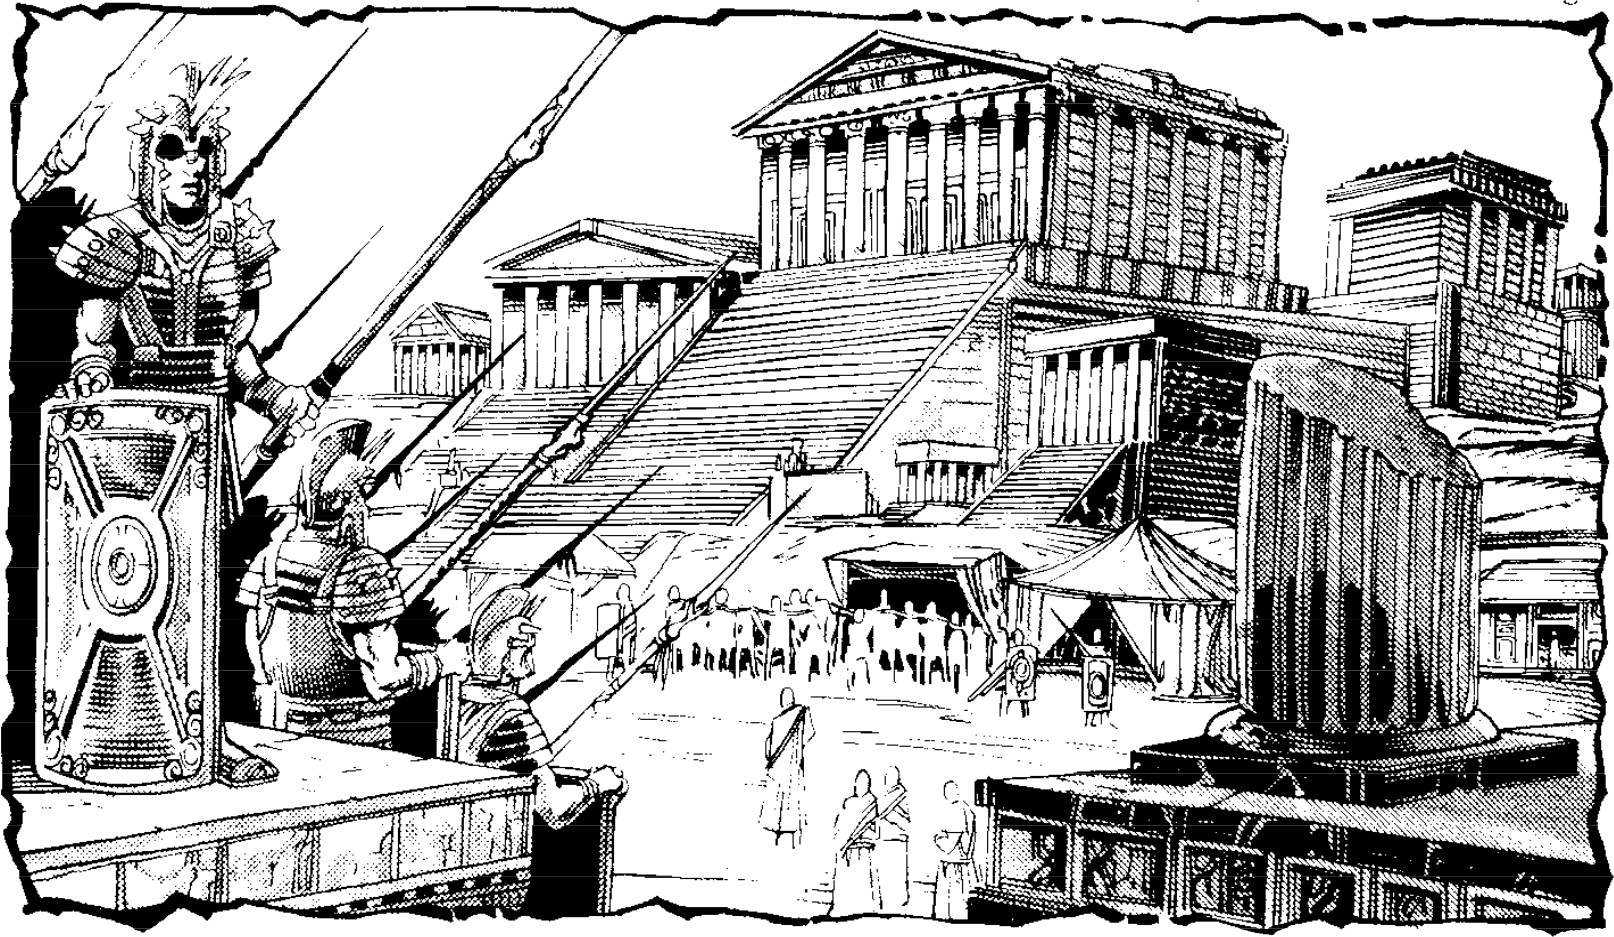
\includegraphics[width=\textwidth]{images/balic-2.png}
\end{figure*}

	After Andropinis' imprisonment, Balic was divided into three parts, each controlled by a different trade lord. These parts cooperate on one level but battle for supremacy on all others.

	The largest block of control falls to Lord Tabaros of House Wavir (NG male human, aristocrat 7/rogue 8/dune trader 5), while Lord Kaladon of House Tomblador (LE male human, rogue 8/dune trader 5) and Lady Essen of House Rees (LN female human, rogue 7/dune trader 5/telepath 4) control equally sized smaller blocks. The same amount of cooperation that allows the three rivals to jointly maintain the major trading village of Altaruk allows them to keep Balic running as a major city-state.

	As far as outsiders are concerned, the three leaders formed a triune council to rule the city after Andropinis fell. While such a council does exist, and the three rivals meet regularly to keep the city-state strong enough to stand against invaders, they each work behind the scenes to build their own power bases up and knock their rivals down.

	Each trade lord has a different view of the world and the way Balic should be governed. Wavir, for example, wants to free all slaves, outlaw defilers, welcome preservers into society, and set up a true democratic state. The way to accomplish this, Lord Tabaros believes, is by quick action and harsh measures. Unfortunately, Tabaros is more than 100 years old and may not be able to stay in power much longer. Publicly, the trade lord appears as sharp and healthy as ever, but privately he suffers the weaknesses of age and illness. He had hoped to pass leadership to his son long ago, but his son died when raiders attacked his caravan in FY 6. The next likely candidate, Tabaros' granddaughter Tarinne (NG female human, fighter 4/rogue 2/dune trader 4), isn't ready for the responsibilities yet (or so Tabaros believes).

	Lord Kaladon wants to resume the dictatorship---with himself as king of Balic. Lady Essen, meanwhile, believes that the city-state should be nothing more than a glorified merchant village, serving to fill the coffers of House Rees and making it the most powerful merchant house in the entire Tyr Region. Needless to say, none of the sides want to see any other gain a significant advantage.

	Those templars who agreed to swear allegiance to one of the trade lords have been retained for their bureaucratic skills. However, the merchant houses have their own administrators to fall back on, so any templars who can't be trusted are eliminated. (A small number of templars still loyal to Andropinis have gone into hiding and continue to work in secret, though they have little power and few hopes of gaining any under the current system.)

	The patricians are allowed varying degrees of participation in the government, depending upon which merchant house holds sway over the territory their land occupies. Under Wavir's control, the patricians are allowed full participation rights. Under House Tomblador, the patricians are treated barely better than slaves, while House Rees gives them the freedom to handle their own affairs-provided they meet the production quotas Lady Essen has established for each patrician family.
}
{
	Today the city-state has no sorcerer-king to lead it or protect it from the ravages of Athas. Balic has always had a tradition of the illusion of democracy. Andropinis claimed to have been freely elected to his position, the templars were elected to ten-year terms by the free citizens, and even the nobles (called patricians) were allowed to participate in the governmental process by selecting members to attend the Chamber of Patricians on a regular basis. Though this democracy wasn't real, it still taught the people about one possible way a free society could work. When the news spread that Andropinis was gone (he had been imprisoned in the Black by Rajaat), various factions called for a new election.

	The main contenders for the position of dictator of Balic were Oriol of Magestalos, First Speaker of the Patricians (LN male human, telepath 7); General Zanthiros of the Balican army (LE male human, fighter 13); and First Templar Asthira (LE female human, templar 6/shadow templar 7). Before the final votes could be counted, Tabaros, the patriarch of House Wavir, made his move. The merchant house seized the White Palace, the silt harbor, and all of the territory in between and declared Tabaros to be the Trade Lord of Balic. This didn't sit well with House Wavir's rivals. Neither House Tomblador nor House Rees wanted to be cut out of this opportunity, so each of these merchant dynasties took over the remaining portions of the city.

	\textbf{Shadow Templars}: When the Trade Lords seized power in Balic, many of the templars swore allegiance to one of the Trade Lords. A small number of templars refused to abandon their loyalty to Dictator Andropinis and have gone into hiding. They hope to one day free Andropinis from his prison, and there are rumors that the shadow templars have already developed a means of communicating with the imprisoned sorcerer-king. They work in the shadows, but have many contacts with the templars that have pledged their allegiance to the Trade Lords. First Templar Asthira leads the shadow templars.

	\textbf{The Veiled Alliance}: Like other organizations in Balic, the city's Veiled Alliance is run by an elected leadership. For this reason, a nonwizard leads the Alliance. Ramphion (LG male human, rogue 11) has held his position for 15 years, winning five elections in a row. The next election must occur later this year, and Ramphion may finally give up his role as head of the Alliance. He has strong ties to House Wavir, though House Rees has begun to court the preservers. Ramphion listens to all sides, hoping to play peacemaker if the three factions ever resort to civil war. The Alliance has two other goals at the moment: to turn Balic into a true democratic society, and to find out if the rumors concerning Andropinis are true.
}
{
	\textbf{Altaruk (Village, 620)}: Altaruk is a client village of the merchant houses of Wavir, Rees, and Tomblador. This major trade village is located at the head of Big Fork of the Forked Tongue Estuary. Heavily fortified, a 4.5-meter wall surrounds the village, and 500 free mercenaries defend it. Altaruk is commanded by Arisphistaneles (LG male human, wizard 5/veiled one 6/dune trader 4), a powerful preserver who allows the Veiled Alliance to use the village as a meeting place. The village is regularly attacked by giants from the islands of the Forked Tongue, and the Great Earthquake buried parts of Altaruk beneath rubble from the nearby mountains. As always, the merchant houses of Balic are in the process of rebuilding the village, for it serves as a key deterrent to raiders along this portion of the trade roads. Protection is extended to caravans of other merchant houses, provided they pay the toll as they pass through Altaruk. For caravans, the toll is one gold piece per caravan mount, an exorbitant price that prohibits most merchants from spending more than one day in the village. For individual travelers the toll is one ceramic piece.

	\textbf{Last Port (Hamlet, 200)}: The village of Last Port is surrounded by a silt moat. The village falls under the influence of Balic, but has maintained its independence as much as it can. Aicmenes (LN male human, telepath 9) leads the village. The village is a mix of Dwarven architecture, influenced by the Smokestone clan that makes Last Port its home, and Balic artistry. A small amber mine is the main source of income for the village, though many villagers also provide services for the silt skimmers that stop at the village's small docks.

	\textbf{Walis (Thorp, 120)}: Walis is a small hidden village in the foothills of the Ringing Mountains. From its position atop a high rock spire the village sits on one of the only active gold mines in the Tyr region. The merchant house Tomblador controls the village and keeps the village's defenses as strong as possible. The village can only be reached from the ground by a cargo bucket lowered by the villagers. Besides a large company of soldiers, six defilers are stationed at the village at all times to add to the defenses.
}
{
	\textbf{Agora}: All the merchant houses have their emporiums in the Balican agora. Surrounding the agora is the Elven market.

	\textbf{Criterion}: Balic's gladiator arena sits beneath the stony bluff of the Megaleneon. The Criterion is an architectural marvel, constructed of pure white marble, with great sails rising from the walls to provide shade. The arena floor is rectangular shaped and consists of hexagon-shaped marble slabs. The slabs are 3 meters wide and 9 meters tall and rest on a bed of sand. This unique floor is always uneven since no two adjoining slabs are of the same height, with as much as 3 meters difference between two slabs.

	\textbf{Fort Glamis}: Established and maintained by House Wavir, Fort Glamis is located on the Balic/Ledopolus road and is an important supply center for caravans from Balic on their way to the rest of the Tyr region.

	\textbf{The Shining Bridges}: Ravines, filled with silt, break through the ground around the agora. Monumental bridges made of marble allow access to the agora.

	\textbf{Segovara}: The village of Segovara was a client village of House Rees of Balic. Located southeast of Balic across the Estuary of the Forked Tongue, the village rests inside a small narrow canyon. The village is mainly a collection of huts built against both sides of the canyon walls. Because of the lack of space inside the canyon only one narrow road exists in the cramped village. The villagers manufactured leather goods for House Rees, however their isolated position, without a source of water, left them utterly depended on Rees caravans. In the chaotic aftermath of the trade lords' seizure of power in Balic the village was forgotten and all of the villagers perished. The next time a caravan from House Rees arrives at the village the entire population will rise as faels.
}
{
	\item Working in secret, a group of templars attempts to open a portal to Andropinis' prison in the Black. Unfortunately for the templars, they were duped by an extraplanar creature into opening a portal to its plane, allowing a band of extraplanar creatures onto Athas. These creatures proceed to run amok throughout Balic. The creatures could be from the Black, one of the elemental planes, or another plane of the DM's choosing.
	\item The animals on House Dagsonius's ranch have begun to talk! The animals do not respond to spoken questions, but randomly blurt out predictions of doom in perfect Balikite to those standing nearby. The head of House Dagsonius is troubled. He raises the animals for slaughter but many in the family do not want to kill the animals if they have become intelligent. He needs someone to get to the bottom of this.
	\item Drake Crag Bay is not far from Balic and takes its name from a rocky crag overlooking the bay that resembles an earth drake. For years the bay has been a prime spot to harvest silt mussels, and many from Balic make their livelihood in the shallow bay. Recently a creature from the deep silt has entered the bay and preys on the mussel harvesters. The creature has remained under the silt so far, so no one is sure what the creature is.
	\item With the current struggle for control of Balic between the three merchant houses being mostly a war in the shadows, the bards of Balic are taking advantage of all sides to generate high profits. When the PCs show up in town, a few of the bards see them as mercenaries who could become competition. The bards try to either force the PCs out of town or eliminate them.
	\item The Silt Blazer, a silt skimmer based out of Balic was three days overdue when it finally sailed into Balic harbor---with no one aboard. There is no sign of the crew; however, the skimmer's cargo appears to be intact. While House Wavir has confiscated the cargo, they hired the PCs to find out what happened to the crew.
	\item As a sign of his status as Dictator, Andropinis did not wear a crown. His position was signified by a rod and cloak, both rumored to be enchanted. The royal regalia disappeared from the Megaleneon in the days after the trade lords seized power. All three trade lords desire the royal regalia to strength their claim to rulership of the city and will pay handsomely for any who recover the items.
}